
% v2-acmsmall-sample.tex, dated March 6 2012
% This is a sample file for ACM small trim journals
%
% Compilation using 'acmsmall.cls' - version 1.3 (March 2012), Aptara Inc.
% (c) 2010 Association for Computing Machinery (ACM)
%
% Questions/Suggestions/Feedback should be addressed to => "acmtexsupport@aptaracorp.com".
% Users can also go through the FAQs available on the journal's submission webpage.
%
% Steps to compile: latex, bibtex, latex latex
%
% For tracking purposes => this is v1.3 - March 2012
\documentclass[prodmode,acmtecs]{acmsmall} % Aptara syntax
\usepackage[spanish,polish]{babel}
\usepackage[T1]{fontenc}
\usepackage{fancyvrb}
\usepackage{graphicx,hyperref}
\newcommand\cutout[1]{}


\usepackage[table]{xcolor}
\usepackage[utf8]{inputenc}
\usepackage[parfill]{parskip}
\usepackage{tabulary}
\PassOptionsToPackage{hyphens}{url}
\usepackage{hyperref}    
\usepackage[capitalize]{cleveref}


% Metadata Information
% !!! TODO: SET THESE VALUES !!!
\acmVolume{0}
\acmNumber{0}
\acmArticle{CFP}
\acmYear{0}
\acmMonth{0}

\newcounter{colstart}
\setcounter{page}{4}

\RecustomVerbatimCommand{\VerbatimInput}{VerbatimInput}%
{
%fontsize=\footnotesize,
fontfamily=\rmdefault
}


\newcommand{\UnderscoreCommands}{%\do\verbatiminput%
\do\citeNP \do\citeA \do\citeANP \do\citeN \do\shortcite%
\do\shortciteNP \do\shortciteA \do\shortciteANP \do\shortciteN%
\do\citeyear \do\citeyearNP%
}

\usepackage[strings]{underscore}



% Document starts
\begin{document}


\setcounter{colstart}{\thepage}

\acmArticle{CFP}
\title{\huge\sc SIGLOG Monthly 229}
\author{DAVID PURSER\affil{University of Warsaw, Poland}
\vspace*{-2.6cm}\begin{flushright}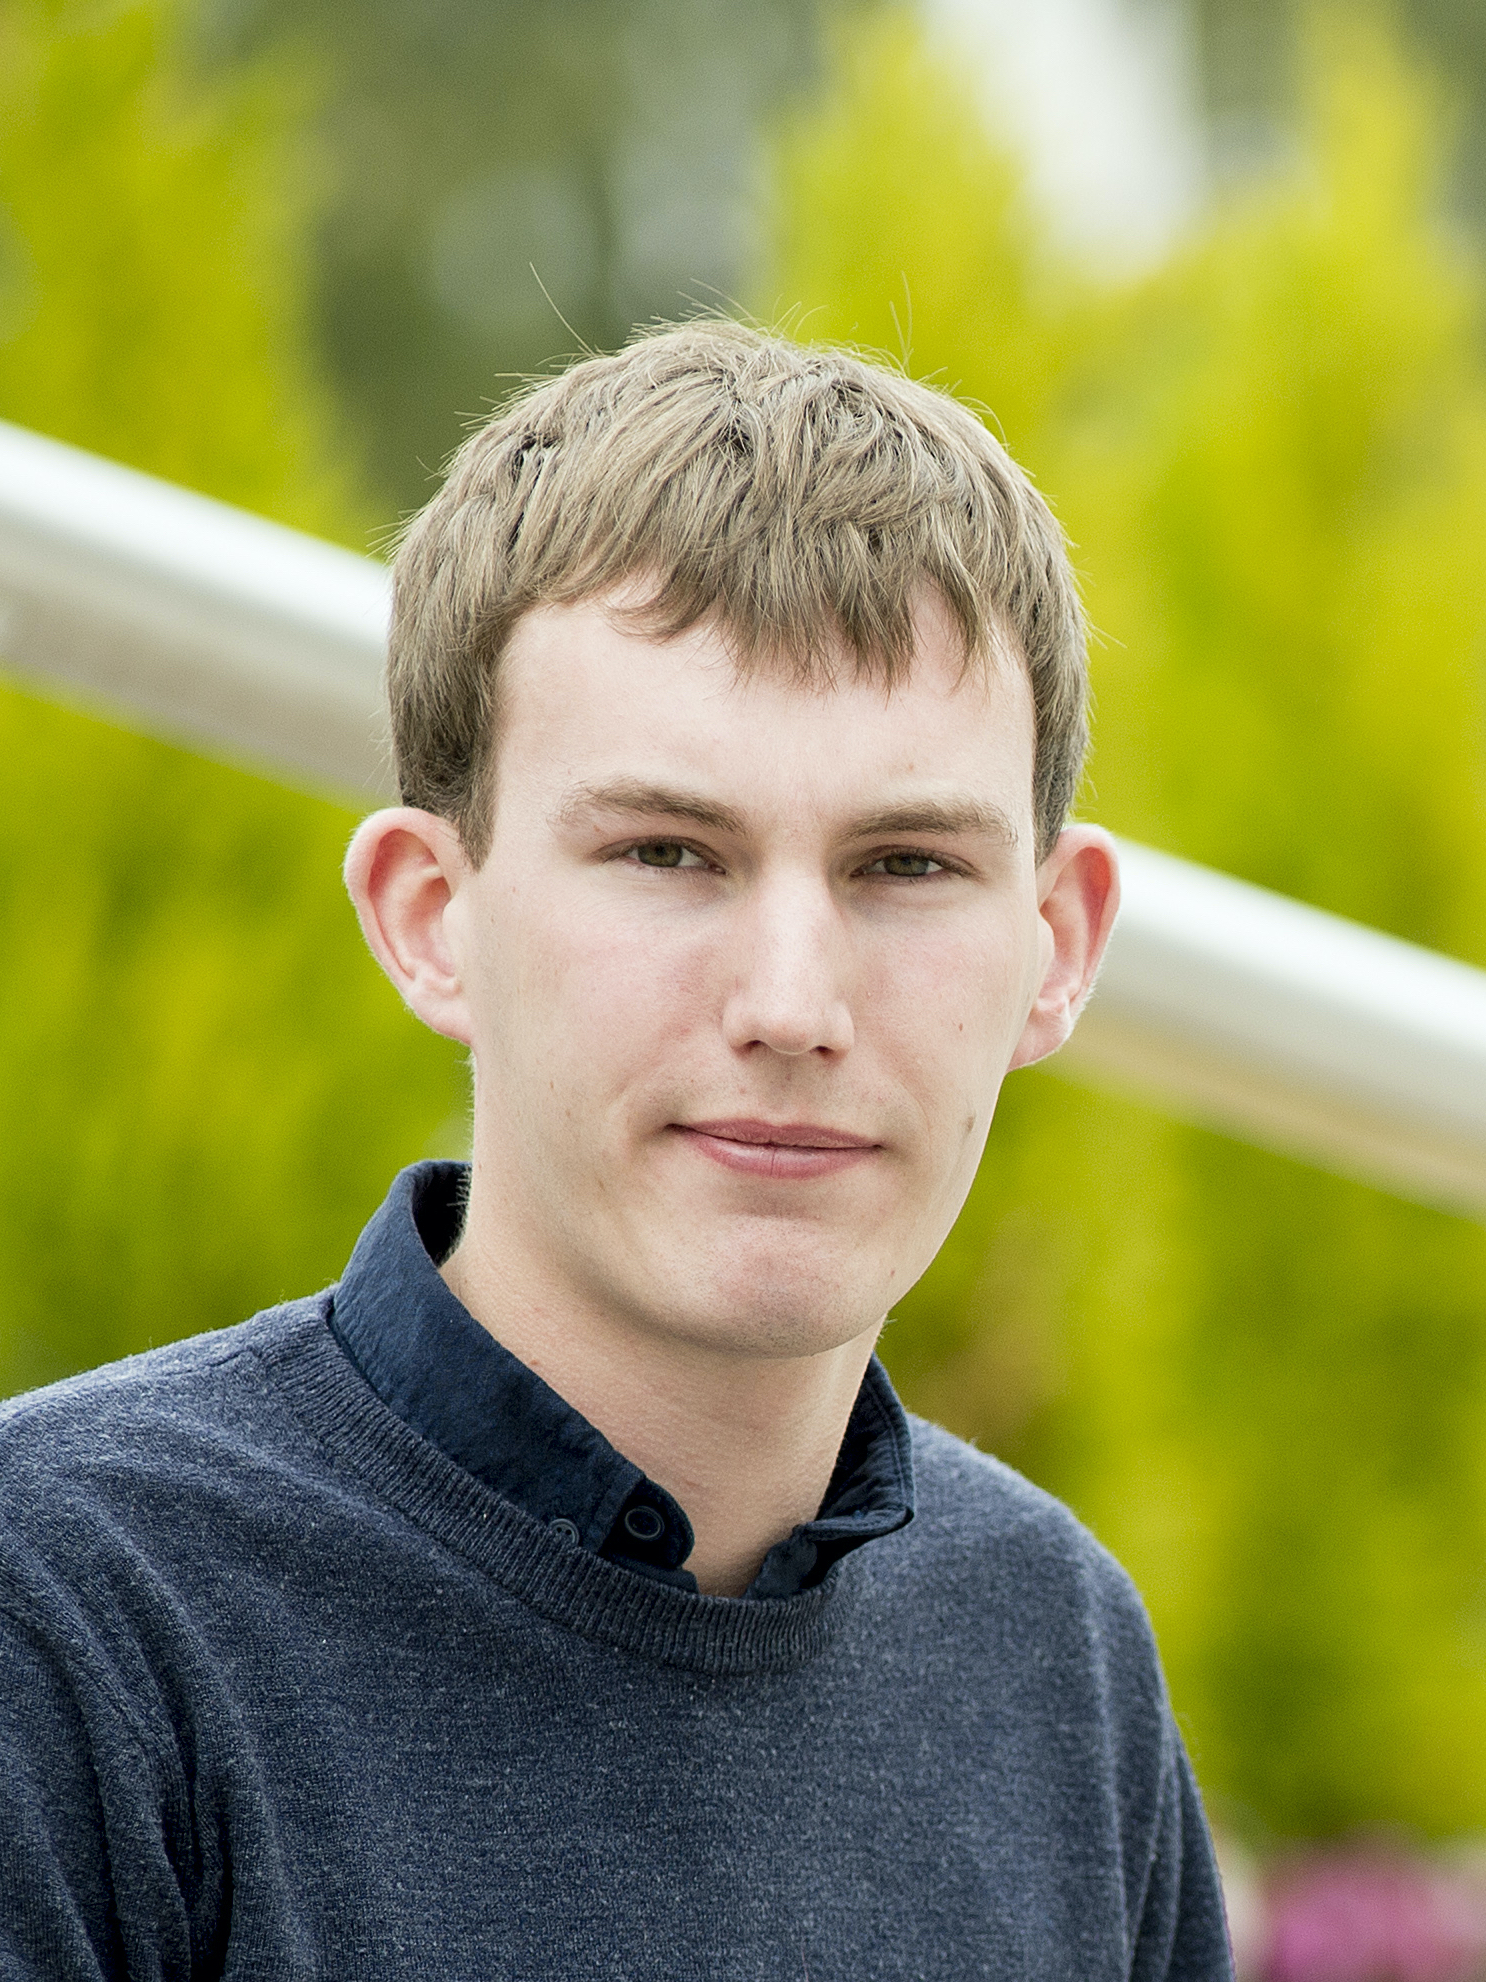
\includegraphics[width=30mm]{dp}\end{flushright}
}

\maketitlee

\href{https://lics.siglog.org/newsletters/}{Past Issues}
 - 
\href{https://lics.siglog.org/newsletters/inst.html}{How to submit an announcement}
\section{Table of Content}\begin{itemize}\item DEADLINES (\cref{deadlines}) 
 
\item CALLS 
 
\begin{itemize}\item CPP 2023 (CALL FOR PAPERS) (\cref{CPP2023})
\item STACS 2023 (CALL FOR PAPERS) (\cref{STACS2023})
\item BEWARE 2022 (CALL FOR PAPERS) (\cref{BEWARE2022})
\item ETAPS 2023 (CALL FOR PAPERS) (\cref{ETAPS2023})
\end{itemize} 
\item JOB ANNOUNCEMENTS 
 
\begin{itemize}\item Lecturer/Senior Lecturer at UNSW, Sydney (\cref{LecturerSeniorLectureratUNSWSydney})
\end{itemize} 
\end{itemize}\section{Deadlines}\label{deadlines}\rowcolors{1}{white}{gray!25}\begin{tabulary}{\linewidth}{LL}The ALP Alain Colmerauer Prolog Heritage Prize:  & Sep 02, 2022 (Deadline for nominations) \\
CPP 2023:  & Sep 14, 2022 (Abstract), Sep 21, 2022 (Paper) \\
BEWARE 2022:  & Sep 23, 2022 (Paper) \\
STACS 2023:  & Sep 25, 2022 (Paper) \\
Lecturer/Senior Lecturer at UNSW, Sydney:  & Sep 29, 2022 (Programming Lanugages Job Closing), Oct 12, 2022 (Formal Methods and Logic in Computer Science Job Closing) \\
OVERLAY 2022:  & Sep 30, 2022 (Paper) \\
FSEN 23:  & Oct 07, 2022 (Abstract), Oct 14, 2022 (Paper) \\
ETAPS 2023:  & Oct 13, 2022 (Paper) \\
PODS 2023:  & Nov 28, 2022 (Second cycle abstract), Dec 05, 2022 (Full paper) \\
\end{tabulary}
\section{CPP 2023: Certified Programs and Proofs}\label{CPP2023}  January 16-17, 2023 \\ 
  Boston, United States\\ 
  \href{https://popl23.sigplan.org/home/CPP-2023#Call-for-Papers}{https://popl23.sigplan.org/home/CPP-2023\#Call-for-Papers}\\ 
CALL FOR PAPERS 

\begin{itemize}\item  Certified Programs and Proofs (CPP) is an international conference on practical and theoretical topics in all areas that consider formal verification and certification as an essential paradigm for their work. CPP spans areas of computer science, mathematics, logic, and education. 
 
  CPP 2023 (\href{https://popl23.sigplan.org/home/CPP-2023}{https://popl23.sigplan.org/home/CPP-2023}) will be held on 16-17 January 2023 and will be co-located with POPL 2023 in Boston, Massachusetts, United States. CPP 2023 is sponsored by ACM SIGPLAN, in cooperation with ACM SIGLOG. 
 
  CPP 2023 will welcome contributions from all members of the community. The CPP 2023 organizers will strive to enable both in-person and remote participation, in cooperation with the POPL 2023 organizers. 
 
\item  IMPORTANT DATES (Strict, AoE) 
 
\rowcolors{1}{white}{gray!25}\begin{tabulary}{\linewidth}{LL}Abstract submission:  & Sep 14, 2022 \\
Paper submission:  & Sep 21, 2022 \\
Notification (tentative):  & Nov 21, 2022 \\
Camera Ready Deadline (tentative):  & Dec 12, 2022 \\
Conference:  & Jan 16-17, 2023 \\
\end{tabulary}
 
\item  DISTINGUISHED PAPER AWARDS 
 
  Around 10% of the accepted papers at CPP 2023 will be designated as Distinguished Papers. This award highlights papers that the CPP program committee thinks should be read by a broad audience due to their relevance, originality, significance and clarity. 
 
\item  TOPICS OF INTEREST 
 
  We welcome submissions in research areas related to formal certification of programs and proofs. The following is a non-exhaustive list of topics of interest to CPP: 
 
\begin{itemize}\item certified or certifying programming, compilation, linking, OS kernels, runtime systems, security monitors, and hardware; 
\item certified mathematical libraries and mathematical theorems; 
\item proof assistants (e.g, ACL2, Agda, Coq, Dafny, F*, HOL4, HOL Light, Idris, Isabelle, Lean, Mizar, Nuprl, PVS, etc); 
\item new languages and tools for certified programming; 
\item program analysis, program verification, and program synthesis; 
\item program logics, type systems, and semantics for certified code; 
\item logics for certifying concurrent and distributed systems; 
\item mechanized metatheory, formalized programming language semantics, and logical frameworks; 
\item higher-order logics, dependent type theory, proof theory, logical systems, separation logics, and logics for security; 
\item verification of correctness and security properties; 
\item formally verified blockchains and smart contracts; 
\item certificates for decision procedures, including linear algebra, polynomial systems, SAT, SMT, and unification in algebras of interest; 
\item certificates for semi-decision procedures, including equality, first-order logic, and higher-order unification; 
\item certificates for program termination; 
\item formal models of computation; 
\item mechanized (un)decidability and computational complexity proofs; 
\item formally certified methods for induction and coinduction; 
\item integration of interactive and automated provers; 
\item logical foundations of proof assistants; 
\item applications of AI and machine learning to formal certification; 
\item user interfaces for proof assistants and theorem provers; 
\item teaching mathematics and computer science with proof assistants.
\end{itemize} 
\item  SUBMISSION GUIDELINES 
 
  Please see the full call for comprehensive information about submission guidelines, publication, copyright and open access. 
 
\end{itemize}\section{STACS 2023: The 40th International Symposium on Theoretical Aspects of Computer Science}\label{STACS2023}  7–10 Mar 2023 \\ 
  Hamburg, Germany\\ 
  \href{https://www.conferences.uni-hamburg.de/event/272/}{https://www.conferences.uni-hamburg.de/event/272/}\\ 
CALL FOR PAPERS 

\begin{itemize}\item   The 40th International Symposium on Theoretical Aspects of Computer Science is planned to take place from 7 March to 10 March 2023 in Hamburg, Germany.  
 
  For the first time, STACS 2023 will consist of two tracks, A and B, to facilitate the work of the program committee(s). 
 
\begin{itemize}\item  Track A is dedicated to algorithms and data structures, complexity and games.
\item  Track B will cover automata, logic, semantics and theory of programming.
\end{itemize} 
\item  LISTS OF TOPICS 
 
  Authors are invited to submit papers presenting original and unpublished research on theoretical aspects of computer science. Typical areas include: 
 
  Track A:  
 
\begin{itemize}\item  algorithms and data structures, including: design of parallel, distributed, approximation, parameterized and randomized algorithms; analysis of algorithms and combinatorics of data structures; computational geometry, cryptography, algorithms for machine learning, algorithmic game theory, quantum algorithms 
\item  complexity, including: computational and structural complexity theory, parameterized complexity, randomness in computation 
\end{itemize} 
  Track B: 
 
\begin{itemize}\item  automata and formal languages, including: automata theory, games, algebraic and categorical methods, coding theory, models of computation, computability 
\item  logic in computer science, including: finite model theory, database theory, semantics, type systems, program analysis, specification \& verification, rewriting and deduction, learning theory, logical aspects of complexity
\end{itemize} 
  These lists are not exhaustive. In particular, both tracks also welcome submissions about current challenges. 
 
\item  SUBMISSION 
 
  Please see the full call for detailed submission information: \href{https://www.conferences.uni-hamburg.de/event/272/page/156-call-for-papers}{https://www.conferences.uni-hamburg.de/event/272/page/156-call-for-papers} 
 
\item  IMPORTANT DATES (AoE) 
 
\rowcolors{1}{white}{gray!25}\begin{tabulary}{\linewidth}{LL}Paper submission:  & Sep 25, 2022 \\
Rebuttal:  & Nov 14-16, 2022 \\
Author notification:  & Dec 04, 2022 \\
Final version:  & Jan 08, 2023 \\
STACS 2023:  & Mar 7-10, 2023 \\
\end{tabulary}
 
\end{itemize}\section{BEWARE 2022: Joint BRIO Workshop (Bias, Risk and Opacity in AI), ME\&E-LP Workshop (Machine Ethics \& Explainability - the Role of Logic Programming), and AWARE AI Workshop (Ethics and AI, a two-way relationship)}\label{BEWARE2022}  Nov 28-Dec 2, 2022,\\ 
  \href{https://sites.google.com/view/beware2022/}{https://sites.google.com/view/beware2022/} \\ 
  Co-located with AIxIA 2022\\ 
  University of Udine, Udine, Italy\\ 
CALL FOR PAPERS 

\begin{itemize}\item  The workshop invites submissions from computer scientists, philosophers, economists and sociologists wanting to discuss contributions ranging from the formulation of epistemic and normative principles for AI, their conceptual representation in formal models, to their development in formal design procedures and translation into computational implementations. 
 
\item  TOPICS  
 
  Topics of interest include, but are not at all limited to: 
 
\begin{itemize}\item  Conceptual and formal definitions of bias, risk and opacity in AI
\item  Epistemological and normative principles for fair and trustworthy AI
\item  Ethical AI and the challenges brought by AI to Ethics
\item  Explainable AI
\item  Uncertainty in AI
\item  Ontological modelling of trustworthy as opposed to biased AI systems
\item  Defining trust and its determinants for implementation in AI systems
\item  Methods for evaluating and comparing the performances of AI systems
\item  Approaches to verification of ethical behaviour
\item  Logic Programming Applications in Machine Ethics
\item  Integrating Logic Programing with methods for Machine Ethics and Explainable AI
\end{itemize} 
\item  SUBMISSION 
 
  The workshop invites (possibly non-original) submissions of FULL PAPERS (up to 15 pages) and SHORT PAPERS (up to 5 pages). Short papers are particularly suitable to present work in progress, extended abstracts, doctoral theses, or general overviews of research projects. Note that all papers will undergo a careful peer-reviewer process and, if accepted, camera-ready versions of the papers will be published on the AIxIA subseries of CEUR proceedings (Scopus indexed). 
 
  Manuscripts must be formatted using the 1-column CEUR-ART Style. For more information, please see the CEUR website \href{http://ceur-ws.org/HOWTOSUBMIT.html}{http://ceur-ws.org/HOWTOSUBMIT.html}. Papers must be submitted through EasyChair \href{https://easychair.org/conferences/?conf=beware22}{https://easychair.org/conferences/?conf=beware22}. 
 
\item  IMPORTANT DATES 
 
\rowcolors{1}{white}{gray!25}\begin{tabulary}{\linewidth}{LL}Paper submission:  & Sep 23, 2022 \\
Notification:  & Oct 21, 2022 \\
Camera ready:  & Nov 18, 2022 \\
\end{tabulary}
 
\item  Organization and Programme Committee: \href{https://sites.google.com/view/beware2022/organization-and-pc}{https://sites.google.com/view/beware2022/organization-and-pc}   
 
\end{itemize}\section{ETAPS 2023: 26th European Joint Conferences on Theory and Practice of Software }\label{ETAPS2023}  Paris, France,  \\ 
  April 22-27, 2023\\ 
  \href{https://etaps.org/2023}{https://etaps.org/2023}\\ 
CALL FOR PAPERS 

\begin{itemize}\item  ABOUT ETAPS  
 
  ETAPS is the primary European forum for academic and industrial researchers working on topics relating to software science. ETAPS, established in 1998, is a confederation of four annual conferences accompanied by satellite workshops. ETAPS 2023 is the twenty-sixth event in the series.  
 
\item  Why choose ETAPS? 
 
\begin{itemize}\item  ETAPS is one of the world's leading fora for research on software science, with a history of more than 25 years. - The proceedings of ETAPS appear in gold open access, with no article processing charge for the authors specifically. 
\item  ETAPS has low participation fees for all and students in particular. 
\end{itemize} 
\item  What is new in 2023? 
 
\begin{itemize}\item The SPIN symposium will be co-located with ETAPS. More info at: \href{https://spin-web.github.io/SPIN2023/}{https://spin-web.github.io/SPIN2023/} . 
\item TACAS will use a double-blind reviewing process.
\item ESOP, FASE, and newly also FoSSaCS welcome voluntary submissions of artefacts for evaluation after paper acceptance; the outcome will not change the paper acceptance decision. 
\item Presentations of the test-of-time-award and the doctoral- dissertation-award winners will take place. 
\item A plenary session for TOOLympics will be organised. 
\end{itemize} 
\item  MAIN CONFERENCES (24-27 April 2023)  
 
\begin{itemize}\item  ESOP: European Symposium on Programming (PC chair: Thomas Wies, New York University) 
\item  FASE: Fundamental Approaches to Software Engineering (PC chairs: Leen Lambers, BTU Cottbus-Senftenberg, and Sebastián Uchitel, University of Buenos Aires) 
\item  FoSSaCS: Foundations of Software Science and Computation Structures (PC chairs: Pawel Sobocinski, Tallinn University of Technology, and Orna Kupferman, Hebrew University of Jerusalem) 
\item  TACAS: Tools and Algorithms for the Construction and Analysis of Systems (PC chairs: Sriram Sankaranarayanan, University of Colorado, Boulder, CO, and Natasha Sharygina, University of Lugano) 
\end{itemize} 
  ETAPS'23 will also host another edition of TOOLympics, organised by Dirk Beyer, Fabrice Kordon, and Arnd Hartmanns.  
 
\item  IMPORTANT DATES (AoE) 
 
\rowcolors{1}{white}{gray!25}\begin{tabulary}{\linewidth}{LL}Paper submission:  & Oct 13, 2022 \\
TACAS artefact submission deadline:  & Nov 10, 2022 \\
Rebuttal (ESOP, FoSSaCS, partially TACAS):  & Dec 6-8, 2022 \\
Paper notification:  & Dec 22, 2022 \\
ESOP, FASE, FoSSaCS artefact submission deadline:  & Jan 05, 2023 \\
Artefact notification TACAS:  & Jan 19, 2023 \\
Paper final version:  & Jan 26, 2023 \\
Artefact notification ESOP, FASE, FoSSaCS:  & Feb 09, 2023 \\
\end{tabulary}
 
\item  SUBMISSION INSTRUCTIONS  
 
  Please see the full call for submssion instructions: \href{https://etaps.org/2023/call-for-papers}{https://etaps.org/2023/call-for-papers} 
 
\item  AWARDS 
 
\begin{itemize}\item  The strongest papers from the four conferences will be nominated for the ETAPS best paper awards of EAPLS, EASST and EATCS, and the SCP best tool paper award.
\item  The ETAPS test-of-time award will be granted, recognising outstanding papers published at ETAPS more than ten years in the past.
\item  The Doctoral Dissertation Award will be granted to promote and recognise an outstanding dissertation in the research areas covered by the four main ETAPS conferences. 
\end{itemize} 
\item  SATELLITE EVENTS (22-23 April 2023)  
 
  A number of satellite workshops and other events will take place during the weekend before the main conferences. 
 
  In particular, there will be a PhD student mentoring workshop organised by Caterina Urban and Wolfgang Ahrendt. 
 
\end{itemize}\section{Lecturer/Senior Lecturer at UNSW, Sydney}\label{LecturerSeniorLectureratUNSWSydney}JOB ANNOUNCEMENT 

\begin{itemize}\item The School of Computer Science and Engineering at UNSW, Sydney has the following open positions at Lecturer/Senior Lecturer (= US Assistant-Associate Professor) level.  
 
\item  Programming Languages, with particular interest in the design and implementation of programming languages, semantics of programming languages, language-based security, programming systems (e.g. virtual machines and run-time systems), compilers, and program analysis, including both theory and tool development.  
 
  \href{https://external-careers.jobs.unsw.edu.au/cw/en/job/509942/lecturersenior-lecturer-in-computer-science-programming-languages}{https://external-careers.jobs.unsw.edu.au/cw/en/job/509942/lecturersenior-lecturer-in-computer-science-programming-languages} 
 
Programming Lanugages Job Closing: Sep 29, 2022 
 
\item  Formal Methods and Logic in Computer Science, with particular interest in algorithmic verification and applications towards areas including security foundations, distributed computing, hybrid systems and autonomous systems.  
 
  \href{https://external-careers.jobs.unsw.edu.au/cw/en/job/510701/lecturer-senior-lecturer-in-computer-science-formal-methods-and-logic}{https://external-careers.jobs.unsw.edu.au/cw/en/job/510701/lecturer-senior-lecturer-in-computer-science-formal-methods-and-logic}  
 
Formal Methods and Logic in Computer Science Job Closing: Oct 12, 2022 
 
\end{itemize}


To the \href{http://siglog.org/}{SIGLOG} or \href{https://lics.siglog.org}{LICS} website\end{document}